\documentclass[11pt,twoside]{article}
\addtolength{\textwidth}{0.5in}
\usepackage{epsfig,amsfonts,color}
\usepackage{amsmath}
\bibliographystyle{plain}
\usepackage{amssymb, palatino, geometry,url}
\usepackage{algorithmic}
\usepackage[noresetcount,lined,boxed]{algorithm2e} % ... for algorithms
\usepackage[colorlinks=true,linkcolor=blue,citecolor=blue,urlcolor=blue]{hyperref}
\geometry{letterpaper,
          left       = 0.9in,
          right      = 0.9in,
          top        = 0.9in,
          bottom     = 0.9in}
\linespread{1.2}

\usepackage{fancyhdr}
\usepackage{enumerate}
\usepackage{float}
\usepackage{subcaption}
\usepackage{graphicx}
\usepackage{caption}
\newcommand{\twopart}[4]
{
	\left\{
		\begin{array}{ll}
			#1 & \mbox{ } {\textrm{#2}} \\
			#3 & \mbox{ } {\textrm{#4}}
		\end{array}
	\right.
}

\newcommand{\N}{\mathbb{N}}
\newcommand{\Z}{\mathbb{Z}}
\newcommand{\Q}{\mathbb{Q}}
\newcommand{\R}{\mathbb{R}}
\usepackage{lineno}
%\linenumbers

\begin{document}

\title{Analysis of Multi-Scale Energy Markets using Stochatic Optimization Techniques}

\author{\textbf{\textit{ISyE 719 Course Project}}\\ \\Apoorva Sampat and Ranjeet Kumar\\
 {\small Department of Chemical and Biological Engineering}\\
 {\small \;University of Wisconsin, 1415 Engineering Dr, Madison, WI 53706, USA}}
\date{}
\maketitle

\begin{abstract}

Electricity markets operate at multiple timescales (from hours to milliseconds) to ensure that supply and demands are matched in real time. These markets involve uncertainties because future electricity prices and demands are unknown at the time of decision-making, e.g. energy sale and purchase commitments by generators. We use stochastic programming techniques to study flexibility and economic opportunities provided by a battery in these markets, namely day-ahead (1-hour timescale) and real-time (5-minute timescale) markets. In this work we consider uncertainty only in electricity loads and determine optimal participation strategies using methods like receding horizon scheme, dual dynamic programming and *fullproblem (scenario sampling)*. We also determine bounds on expected policy costs by using perfect information and two-stage approximation (with restriction on states). We compare the costs of participation in exclusively in day-ahead market and both day-ahead and real-time markets. Our results show that market participation only in day-ahead energy markets can *significantly* reduce economic flexibility as compared to participating in both levels of markets.
\end{abstract}


\section{Introduction}

Power grids coordinate a diverse set of energy systems (generators, loads, storage devices) to ensure that supply and demands are matched at multiple timescales (from hours to milliseconds). Such coordination is achieved through hierarchical (multi-scale) market transactions. The proportion of transactions occurring at different timescales is changing as more intermittent and non-dispatchable power is injected into the system.  For instance, wind power introduces power injection fluctuations at high frequencies, which require adjustments in fast real-time energy and ancillary services markets (regulation)  \cite{banakar2008impacts}.  Automation architectures for a broad spectrum of electricity generation and consumption systems (e.g., manufacturing building)  are currently being re-designed to exploit incentives provided by faster and more volatile energy markets. For example, the Alcoa Point Comfort Power Plant, which is a utility plant that provides electricity and steam to the adjacent aluminum manufacturing facility, re-optimizes its operations every 15 minutes in response to electricity and natural gas price fluctuations  \cite{Valadez2008}. These new flexibility-oriented automation architectures provide load flexibility to the power grid in exchange for monetary payments or deferred costs. Similarly, large-scale battery systems and building systems are becoming key providers of dynamic flexibility to the power grid \cite{Hao2012,Fares2014}. 

\subsection{Electricity Markets and Demand Response}

Understanding the economic incentives provided by generation and load flexibility requires of careful consideration of wholesale electricity market structures and diverse products. Figure \ref{fig:market_control_structure} shows the multiscale control structure currently used to balance the power grid. Resources can participate by buying/selling electrical energy and/or providing ancillary services (regulation, reserves). Figure \ref{fig:energy_AS_prices} shows time-varying prices from the California Independent System Operator (CAISO) for three consecutive days. Energy is transacted at three timescales: in the integrated forward market (day-ahead market with 1-hour intervals), in the fifteen minute market, and through the real-time dispatch process (5-minute intervals). Table \ref{tab:caiso_products} lists the different products transacted at each timescale. Histograms for energy prices at different markets are presented in Figure \ref{fig:CAISO_prices2}. As can be seen, prices are less volatile in the day-ahead market and the average price is higher. In the real-time market (FMM, RTD) prices are frequently negative and occasionally exceed \$150/MWh. Energy systems with fast dynamics (e.g., flywheels, batteries) can exploit these fast price fluctuations.

In the U.S., generators/loads provide the hierarchical market structure with addition flexibility via \emph{regulation} and \emph{reserve} ancillary service products. Generators and loads providing regulation capacity permit the power Automatic Generator Control (AGC) layer (run by the ISO or similar grid entity) to adjust their load set-point with a specified range \cite{Jaleeli1992}. Depending on market region, the AGC layer updates load set-points every 2 to 15 seconds. The regulation service provider is compensated both for the amount of regulation capacity provided (a load flexible \emph{band} is offered) and the amount of \emph{mileage}, which is the sum of the absolute distance between consecutive load set points. Mileage calculations are illustrated in Figure \ref{fig:reg_mileage}.  Order 755 of the Federal Energy Regulatory Commission (FERC) provides incentives to participants capable of tracking fast changing load set-points. In California, regulation services are procured as two separate products, regulation up and regulation down, depending on the direction of the flexibility band relative to the nominal set-point (from the corresponding energy market). Spinning reserves support regulation service and safeguard against unplanned outages and increased loads. Spinning reserves are rarely dispatched and resources providing reserves are compensated for providing flexibility/contingency. As additional intermittent and non-dispatchable wind and solar power is absorbed, balancing the power grid becomes more challenging due to high-frequency (minute) variations from these sources. As such, requirements for ancillary services are expected to grow. For example, regulation capacity requirements for Texas are anticipated to increase by 10 to 15\% if wind penetration increases from 5,000 MW to 15,000 MW \cite{Walling2008}. In February 2016, CAISO approximately doubled regulation capacity requirements to account for non-dispatchable renewable sources. As consequence the market price for regulation doubled, resulting in a combined quadrupling of payments to some regulation providers \cite{RTO_Insider}. Finally, reductions in the supply of ancillary services are expected with the retirement of coal-fired generators \cite{Kirby2011}, creating additional opportunities for flexible load providers.

Manufacturing facilities and other large electricity consumers may also participate in electricity markets through Demand Response (DR) programs by manipulating their loads and/or by using on-site generators. DR is typically classified as dispatchable and non-dispatchable, as shown in Figure \ref{fig:DR_classifications}. For dispatchable DR, the ISO directly controls the load (e.g., balancing authority sends new set points through AGC system to regulation resources), whereas non-dispatchable loads are coordinated through a variety of pricing signals including real-time electricity markets, which are updated every 5 to 15 minutes. In Texas, load resources provide 2,400 MW of energy and ancillary services, including half of the spinning reserve capacity. To give an idea of the impact of manufacturing, around 1,000 MW of this capacity is obtained from a single electrochemical processing facility that provides regulation and other services. Medium (10 to 50 MW each) and small (less than 10 MW) size industrial/commercial facilities provide the remaining 820 MW and 550 MW of capacity, respectively \cite{Kirby2011}. The Alcoa facility in Warrick, IN offers several ancillary services in markets run by the Midcontinent ISO. The aluminum smelter provides 70 MW of regulation capacity, which is 15\% of its average load (470 MW). This type of operation represents a paradigm shift on the use of manufacturing loads for ancillary services. The same plant also provides 75 MW of interruptible load, which has been dispatched around 55 times per year for an average length of 42 minutes  \cite{Todd2009,Todd2013}. Alcoa generates up to {\em 120,000 \$/day of additional revenue by participating in electricity markets}, and has identified potential for 10\% energy cost reductions through more targeted operations \cite{Todd2013}. Based on data from CAISO, a system providing 10 MW of regulation capacity for every hour in 2015 would have received 500,000 \$/year plus mileage payments. Regulation capacity prices currently reach up to 59 \$/MW and this number might increase as more renewable power is adopted. Moreover, shifting 10 MW of load during the 1\% most extreme prices (in the 97 to 1,621\$/MWh range) in the CAISO real-time energy market to the average price (30 \$/MWh) would yield savings of 400,000 \$/yr. The savings for large manufacturing facilities can reach millions of dollars per year. For instance, the pumping system of an oil pipeline comprised of 50 pump units with 6,500 horsepower electric motors has a load of 200 MW. Large refineries in Texas have generation facilities of up to 500 MW and usually have excess power capacity installed 
%%%%%%%%%%%%%%%%%%%%%%%%%%%%%%%%%%%%%%%%%%

\section{Decision-Making Setting}\label{sec:setting}
The rechargeable Li-ion batteries can be inter-connected to the power grid to provide electricity and regulation services to the grid. Electricity services imply that batteries can provide power to or draw power from the grid. Power drawn from or provided by the grid to batteries can be regulated within a certain regulation capacities (a "regulation band"). The operator of the power grid (which is called an Independent System Operator or ISO) compensates the battery-owners for both the electricity and regulation services. The goal for the battery-owners is to maximize the revenues generated from both the services.

The electricity markets in California are organized in three levels of time - (1) Day-ahead market, (2) Quarter-hourly market, (3) Real-time market. The  day-ahead market has the time scale of 1 hour, quarter-hourly market has the time scale of 15 minutes and the real-time market has the time scale of 5 minutes. Here, for example, the time scale of the day-ahead market means that the electricity in day-ahead market is traded in intervals of 1 hour with the prices being constant in each interval of 1 hour and varying after the intervals. The price data in the three levels of energy markets for a day have been shown in Figure \ref{eprices}.
\begin{figure}[h!tp]
\centering
\begin{subfigure}[b]{0.32\textwidth} 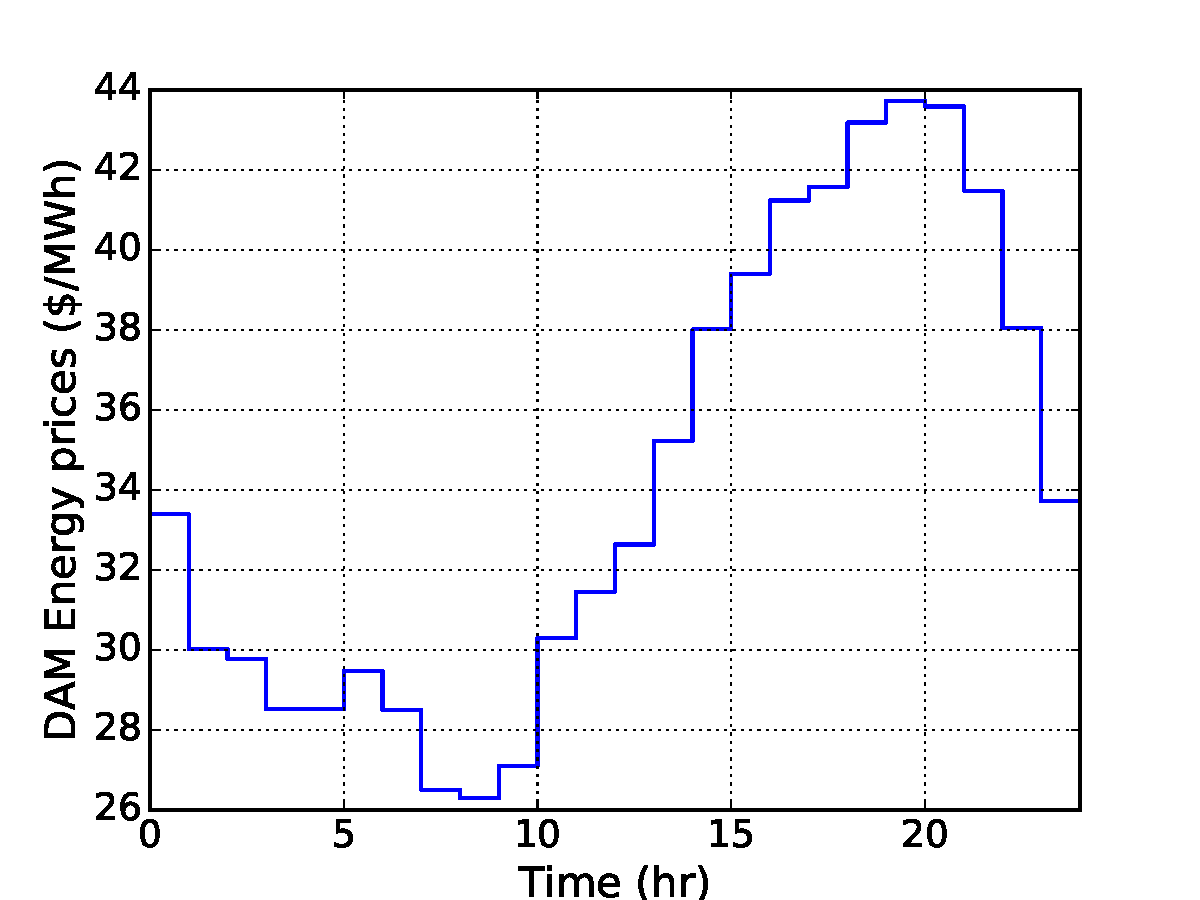
\includegraphics[width=\textwidth]{Figures/damprices.pdf} \caption{Day-ahead market}\label{damprices} \end{subfigure} \hfill
\begin{subfigure}[b]{0.32\textwidth} 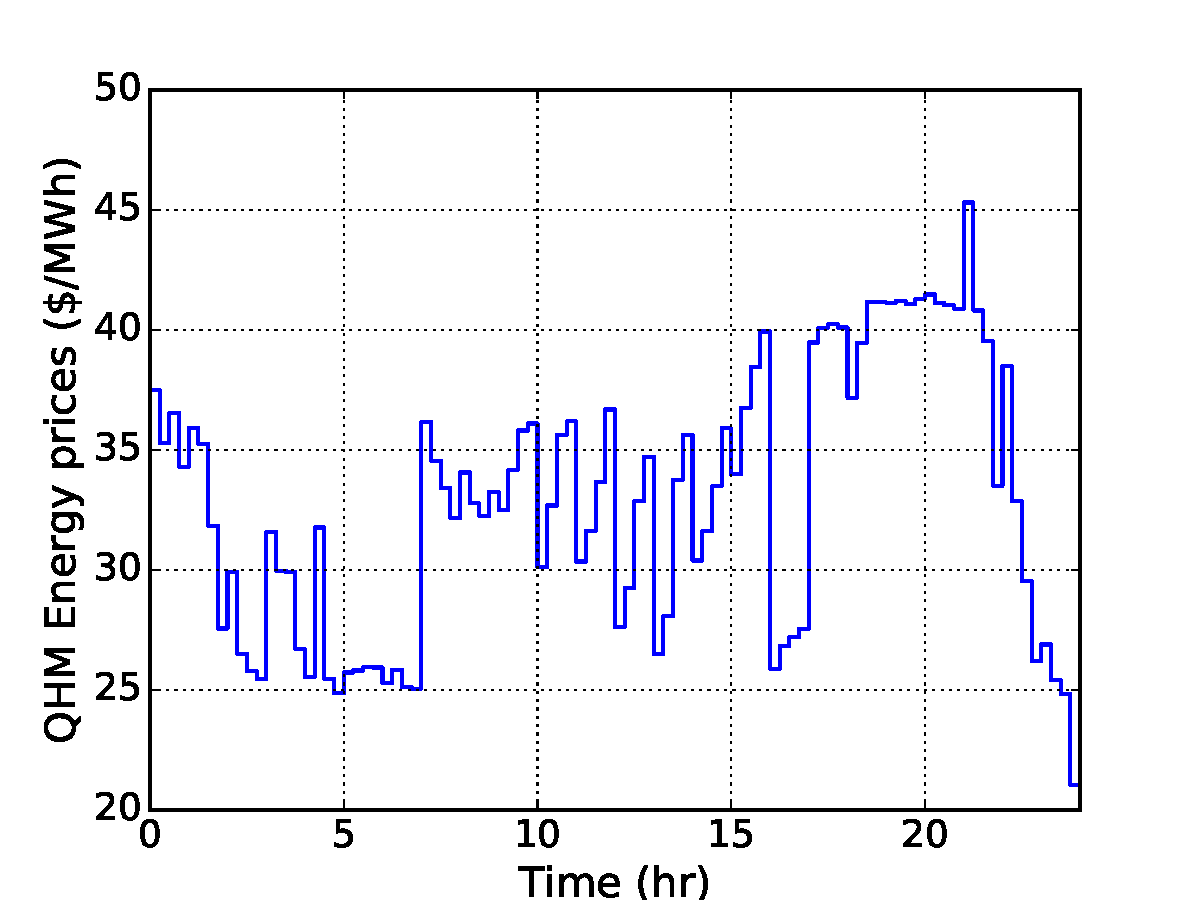
\includegraphics[width=\textwidth]{Figures/qhmprices.pdf} \caption{Quarter-hourly market}\label{qhmprices} \end{subfigure} \hfill
\begin{subfigure}[b]{0.32\textwidth} 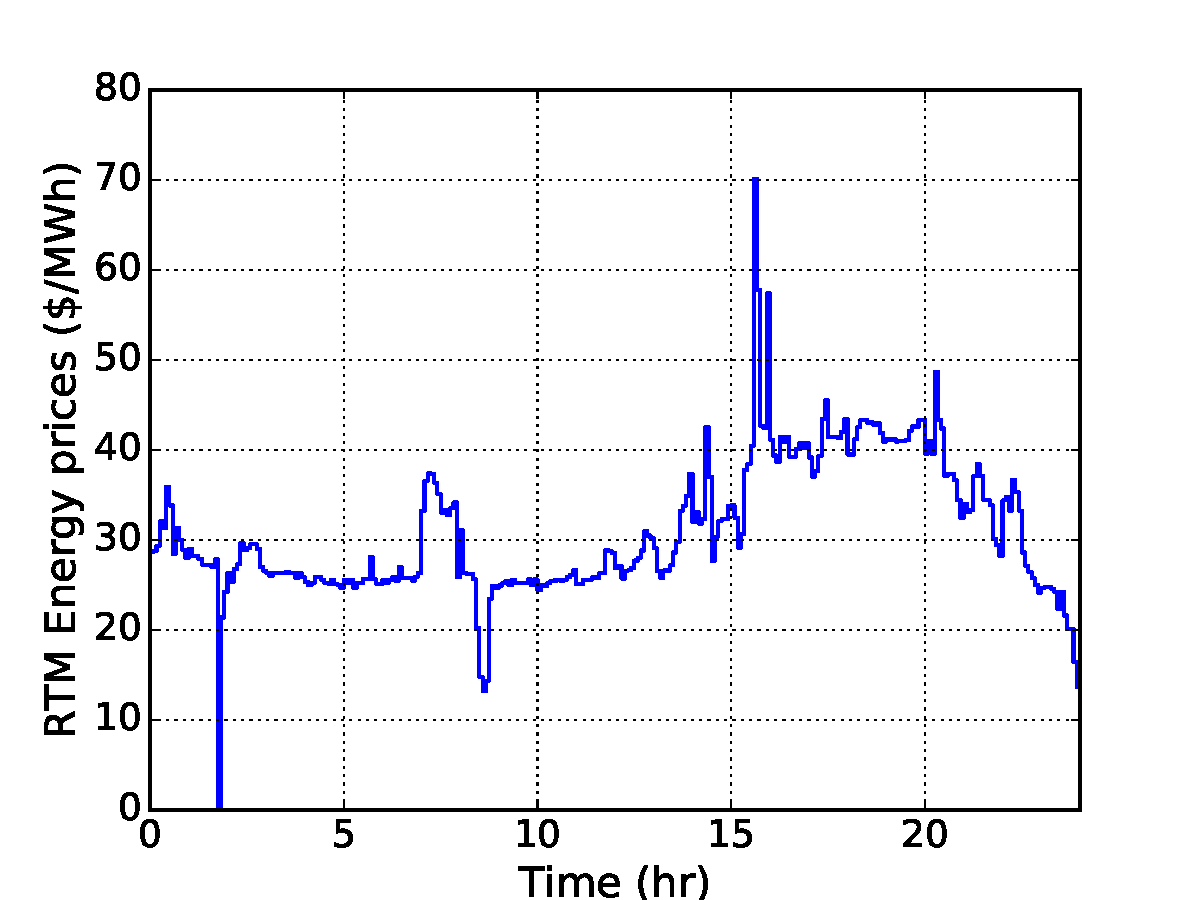
\includegraphics[width=\textwidth]{Figures/rtmprices.pdf} \caption{Real-time market}\label{rtmprices}\end{subfigure} \hfill
\caption{Energy prices in the markets in California}\label{eprices}
\end{figure}
We can observe that there are different frequencies of variation in energy prices in each of the three markets.

On the other hand, the regulation services are traded at two levels of time - (1) Day-ahead market and (2) Quarter-hourly market. The price data in the two levels of regulation markets for a day have been shown in Figure \ref{regprices}.
\begin{figure}[h!tp]
\centering
\begin{subfigure}[b]{0.49\textwidth} 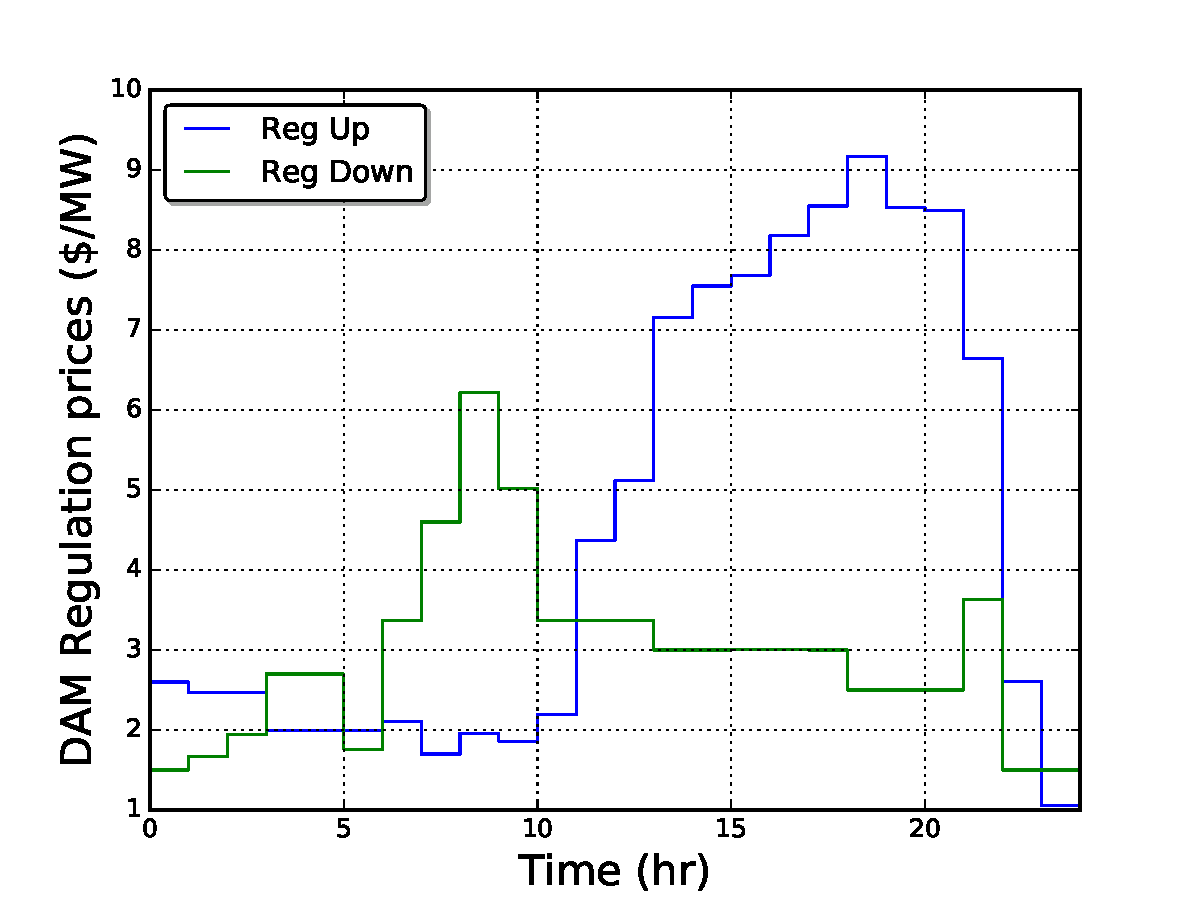
\includegraphics[width=\textwidth]{Figures/DAM_Reg_Price.pdf}\caption{Day-ahead market}\label{damregprices} \end{subfigure} \hfill
\begin{subfigure}[b]{0.49\textwidth} 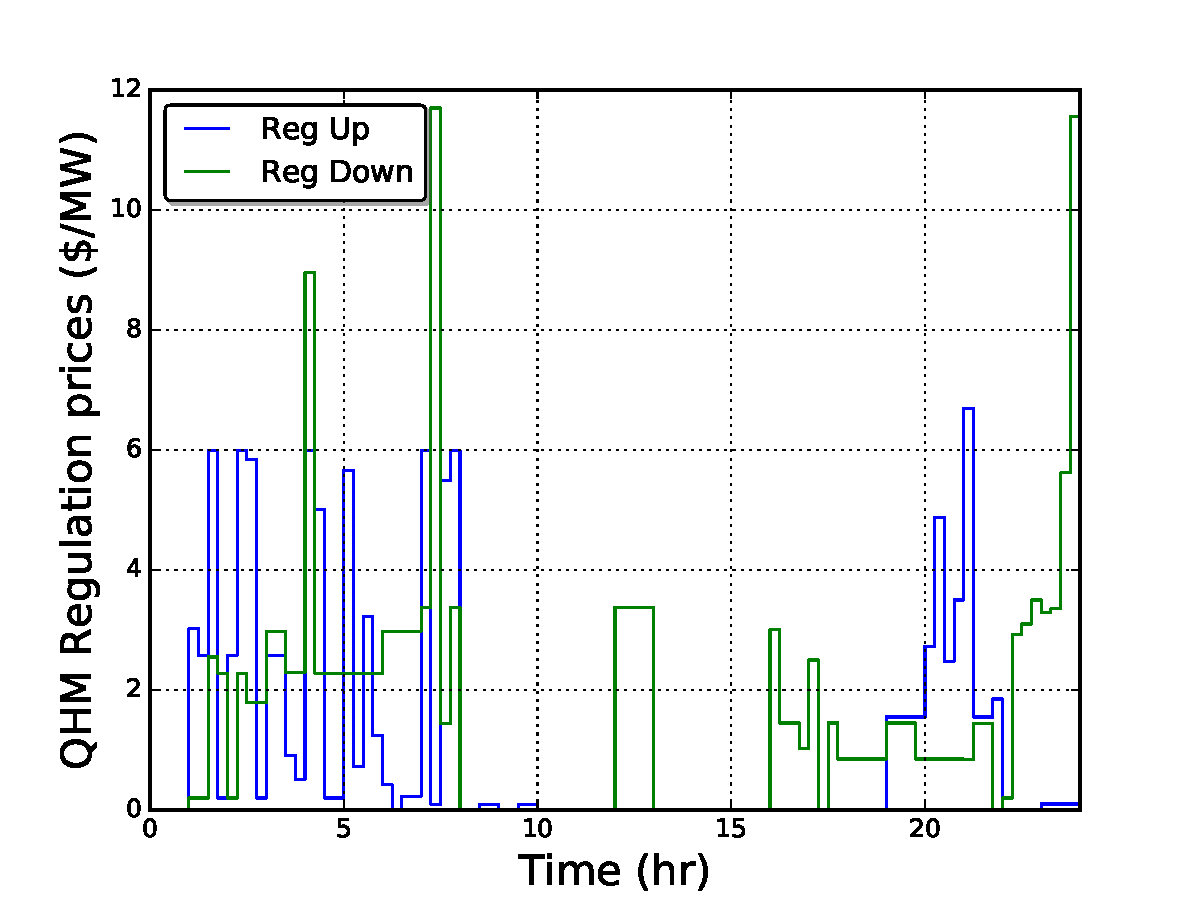
\includegraphics[width=\textwidth]{Figures/QHM_Reg_Price.pdf}\caption{Quarter-hourly market}\label{qhmregprices} \end{subfigure}
\caption{Regualtion prices in the regulation markets in California}\label{regprices}
\end{figure}

Cosidering the price data for a full year to be known (deterministic) we can solve the optimization problem to maximize the annual revenues by operating a battery in the power grid for the whole year. In this work, we aim to solve this deterministic optimization problem with two approaches:
\begin{enumerate}
\item Simultaneous approach: In this approach, we formulate a single giant optimization problem for a full year and solve it to produce the optimal power and regulation capacities that the battery should operate with in each time interval in all the three markets. 
\item Rolling (1 day) horizon approach: In this approach, we formulate an optimization problem for a day and solve it to produce the optimal power and regulation capacities for that day, then take the solutions at the end time-point of that day as the initial point for the next day, then formulate the optimization problem for the next day with those initial values and solve for the second day and sequentially we solve for the 365 days. It is called rolling horizon because in this approach we consider a horizon of 1 day and keep shifting the horizon to to the next day after solving the current day.
\end{enumerate}

At the end, we will compare the two solutions and investigate the advantages and disadvantages of the two approaches.

\section{Illinois Case Study}\label{sec:case}

We use a case study in Illinois to illustrate some of the insights that can be gained with the proposed full-resolution model. The Illinois power grid transmission system  is built on a realistic data set that we have used for previous studies \cite{zavaladispatch}. The system comprises $2{,}522$ lines, $1{,}908$ nodes, $870$ demands points, and $225$ generators points (153 gas-fired generators). Because of the difficulty in obtaining natural gas infrastructure data, we construct a simulated natural gas network system using the basic topology reported by the EIA (see \url{http://www.eia.gov/pub/oil_gas/natural_gas/analysis_publications/ngpipeline/midwest.html}) and by using engineering insight to ensure gas supply to all the gas-fired power plants under nominal conditions. The gas network designed comprises 215 pipeline segments, 157 nodes, 12 compression stations, and 4 supply points. The resulting network in sketched in Figure \ref{gridgas}. 


\subsection{Economic Issues}

We compare economic performance for the infrastructures under coordinated and uncoordinated settings.  We use a time horizon of 24 hours. The results are summarized in Table \ref{table:econ}. In our simulations, the electrical loads were always satisfied; consequently, we report only the generation cost component of the grid cost $\varphi^{grid}$. From the results we make the following observations:
\begin{itemize}
\item Under a coordinated setting the power cost decreases by 0.38\% which represents a total of \$140,000. The gas cost decreases by 7\%, which corresponds to a total of  \$970,000.  
\item Under an uncoordinated setting only 96\% of the gas requested is delivered. {\em At a gas price of 3 \$/MMBTU (see \url{http://www.eia.gov/naturalgas/weekly/}), the total undelivered gas has an economic value of \$599,000.}  
\item Under a coordinated setting the compression cost increases by 17.4\%. This is the result of an increased amount of gas delivered to the power plants. In particular, {\em 7\% more gas is delivered under the coordinated setting.}  At a gas price of 3 \$/MMBTU, the value of the additional gas delivered is \$1,070,000.  Note that the total increase in compression cost is negligible compared to the additional value of the delivered demand.  
\item Under a coordinated setting the revenue for the gas-fired generators increases by  27\%, which corresponds to a total of \$800,000. This the   result of the additional gas delivered and the decreased revenue penalties resulting from coordination. 
\end{itemize}

\begin{table}[htp]
\footnotesize
\caption{Economic performance under coordinated and uncoordinated settings (scm= standard cubic meters and M\$=million U.S. dollars).}
\begin{center}
\begin{tabular}{ccccccc}
                                         &$ \varphi^{grid}$ [M\$] &$ \varphi^{gas}$ [M\$] & $ \varphi^{gas,comp}$ [\$]  & $d^{gas,target} $[scm $\times10^{-6}$] & $d^{gas}$ [scm$\times 10^{-6}$] & $\mathcal{R}$ [M\$]\\
\hline {\bf Uncoord} &         36.54              &        -13.52             &         28,618           &  141.25                & 135.54          & 2.70\\
{\bf Coord}               &        36.40              &        -14.54             &         33,600           &  145.74               &  145.74          & 3.50 
\end{tabular}
\end{center}
\label{table:econ}
\end{table}%

\begin{figure}[h!]
\begin{center}
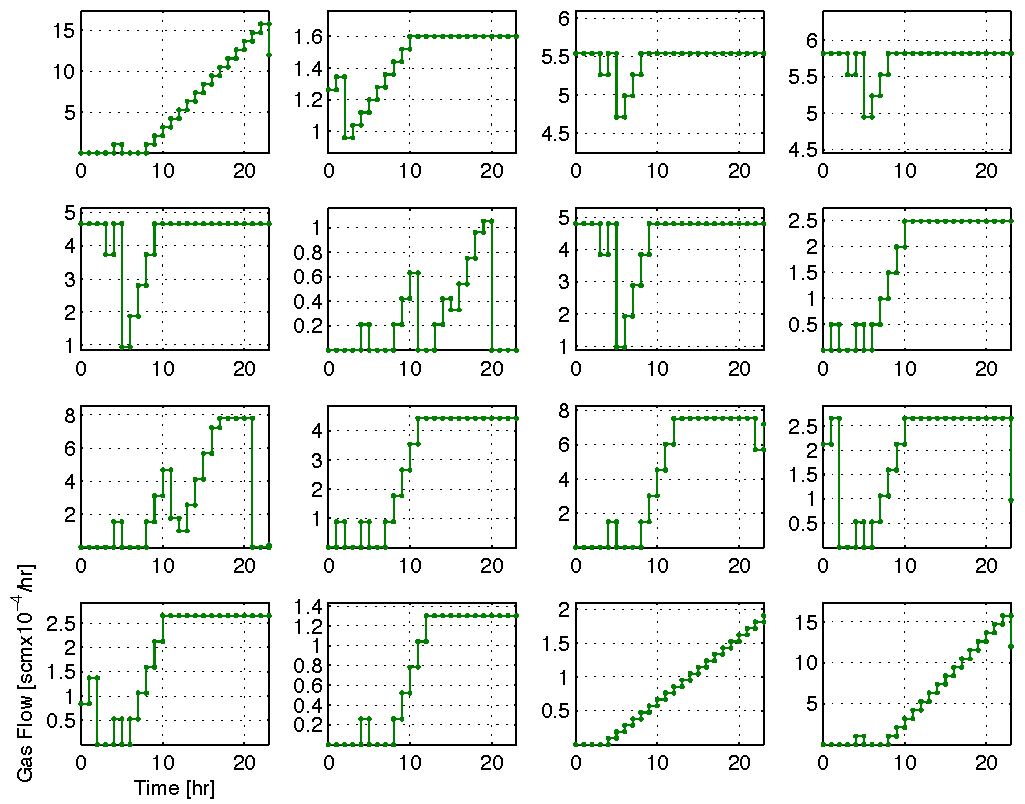
\includegraphics[width=4.5in]{gas_demands_realized_coupled.pdf}\caption{Requested (blue solid line) and realized (green dotted line) gas demands for 16 power plants under coordinated setting.}\label{demands_coupled}
\end{center}
\end{figure}

\begin{figure}[h!]
\begin{center}
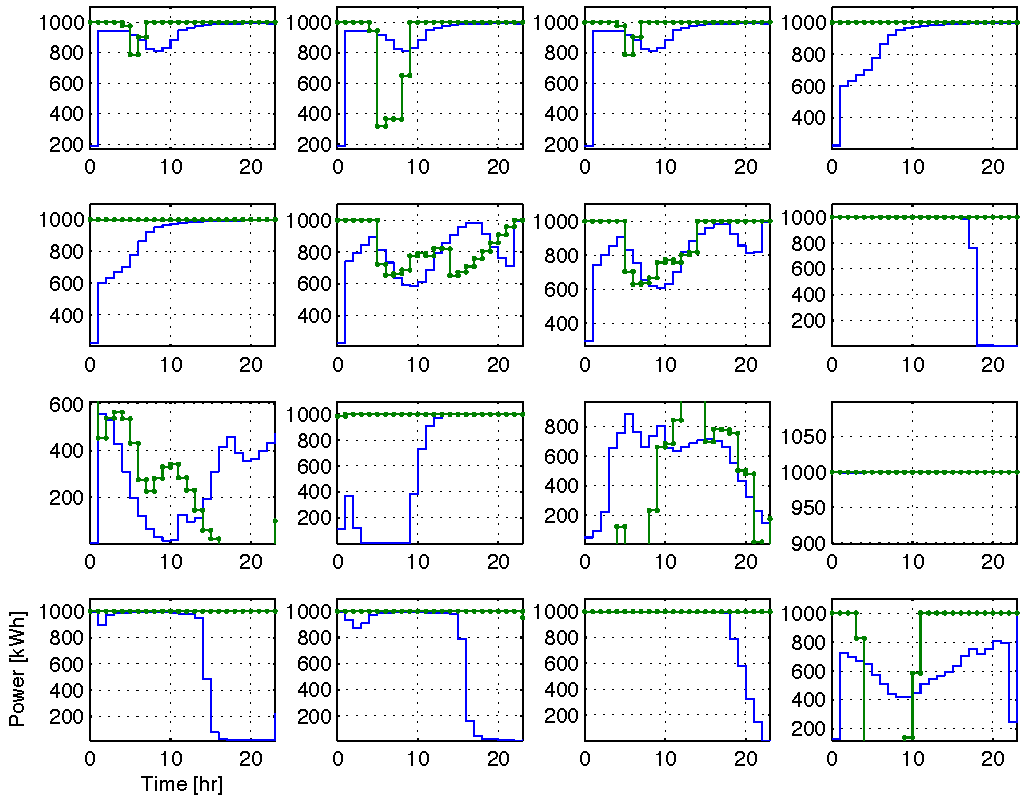
\includegraphics[width=4.5in]{power_coupled_decoupled.pdf}\caption{Power compression profiles under uncoordinated (blue) and coordinated (green) settings for 16 different compressor stations.}\label{power}
\end{center}
\end{figure}

\begin{figure}[h!]
\begin{center}
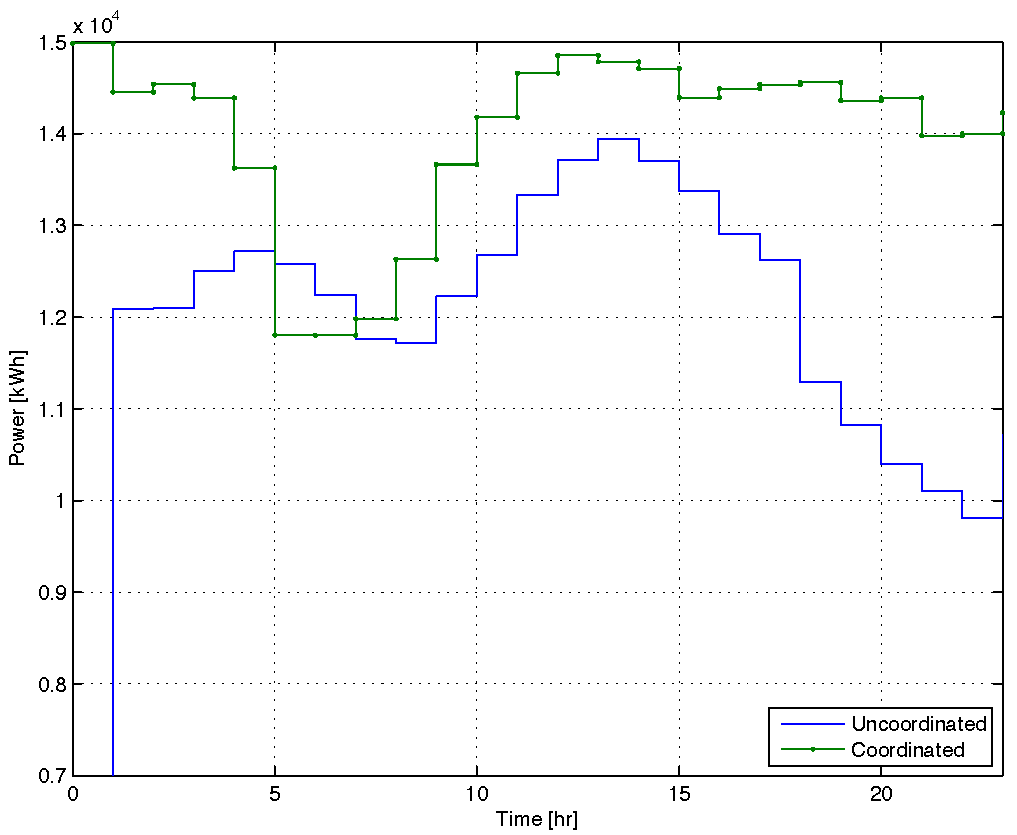
\includegraphics[width=3in]{power_total.pdf}\caption{Total compression power uncoordinated (blue) and coordinated (green).}\label{powertotal}
\end{center}
\end{figure}

It is rather surprising that both the gas and power grid sides benefit from coordination (i.e., {\em the objectives of the gas and grid operators do not compete}). Moreover, gas-fired generators increase their revenue.  We can explain the decreased performance under an uncoordinated setting from the fact that the power grid operator cannot easily determine how much gas can the gas network deliver at different spatial locations and at different times. Thus, the power grid operator can be overly optimistic (as in the case presented) or pessimistic about the amount of gas that can actually be delivered. This situation is clearly illustrated in Figure \ref{demands_decoupled}, where we present the target and realized gas demands for 16 different gas-fired generators for the uncoordinated setting. Note that the gas network cannot deliver the total amount of gas requested at four locations. The resulting error in the prediction introduces a penalty for both the power grid and the gas-fired generators. In particular, the power grid operator has to dispatch more expensive power plants, resulting in higher a generation cost and the power plants have to pay for the unserved generation.  Note also that, {\em even if the gas operator knows the gas demands of the power grid in advance}, it cannot guarantee to satisfy such demands due to physical constraints.  In other words, the spatiotemporal gas demands policies emanating from the power grid dispatch plan can be infeasible to the gas infrastructure. 

From  Figure \ref{demands_decoupled}  we can also see that several gas-fried generators are dispatched  aggressively under an uncoordinated setting (i.e., some gas demands are step functions). This is evident from panels 1, 14, 15, and 16 (the panels are numbered row-wise starting from the upper left corner). Line-pack storage in this case is sufficient to track the steep changes in gas demand. Doing so, however, comes at the expense of decreased flexibility at other locations and this leads to unserved demands.  From panels 1, 14, 15, and 16 of Figure \ref{demands_coupled} we also see that dispatch under a coordinated setting is smoother (i.e., demands are ramps) and this significantly enhances the flexibility to deliver gas at other locations. We observe that, under a coordinated setting, gas-fired generators act as {\em distributed demand response resources}  that the gas operator can use to better control network pressures and flows and thus avoid delivery bottlenecks. In other words, {\em gas-fired power plants become assets rather than liabilities to the pipeline operator.} As a result, all the demand targets can be met and significantly more gas can be delivered compared to the uncoordinated setting. This clearly illustrates the increased physical flexibility gained by coordination.  

Figure \ref{power} presents the compression power profiles under coordinated and uncoordinated settings for 16 different compressor stations. We observe that more compressors operate at full capacity and less variations are observed under a coordinated setting, a situation that is desirable from an efficiency stand-point (i.e., it is inefficient to operate compressors at partial loads and to ramp them up and down continuously from an equipment lifetime and emissions standpoint). From Figure \ref{powertotal} we see that more compression power is used under the coordinated setting because of the increased amounts of gas delivered to the power plants but the compression profile is flatter. 

Figures  \ref{flow_uncoupled}  and \ref{flow_coupled} present axial flow profiles at 16 different pipeline segment for the uncoordinated and coordinated settings, respectively.  Each panel presents the time profiles at 10 different axial positions for a given pipeline segment.  We can see how the different dispatch plans drastically change the flow profiles of the network.  This result indicates that {\em power grid dispatch decisions can significantly influence the spatiotemporal dynamics of the entire gas infrastructure.} 

\begin{figure}[h!]
\begin{center}
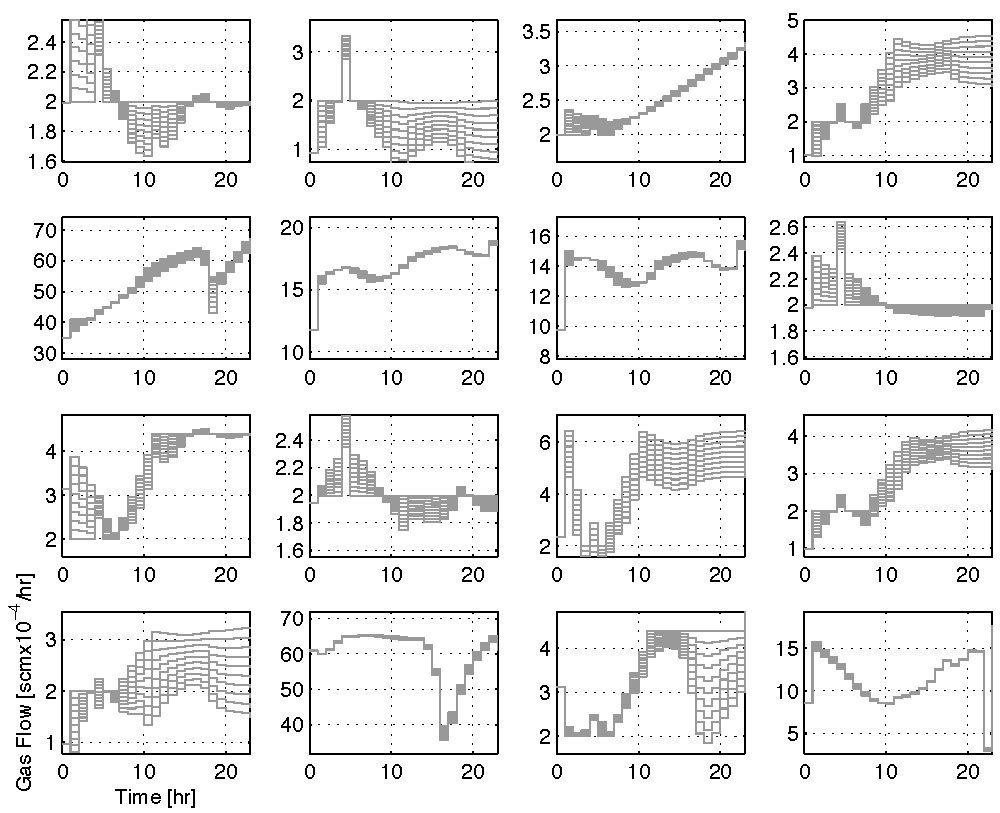
\includegraphics[width=4in]{flow_decoupled.pdf}\caption{Spatiotemporal flow profiles for 16 different pipeline segments for uncoordinated setting.}\label{flow_uncoupled}
\end{center}
\end{figure}

\begin{figure}[h!]
\begin{center}
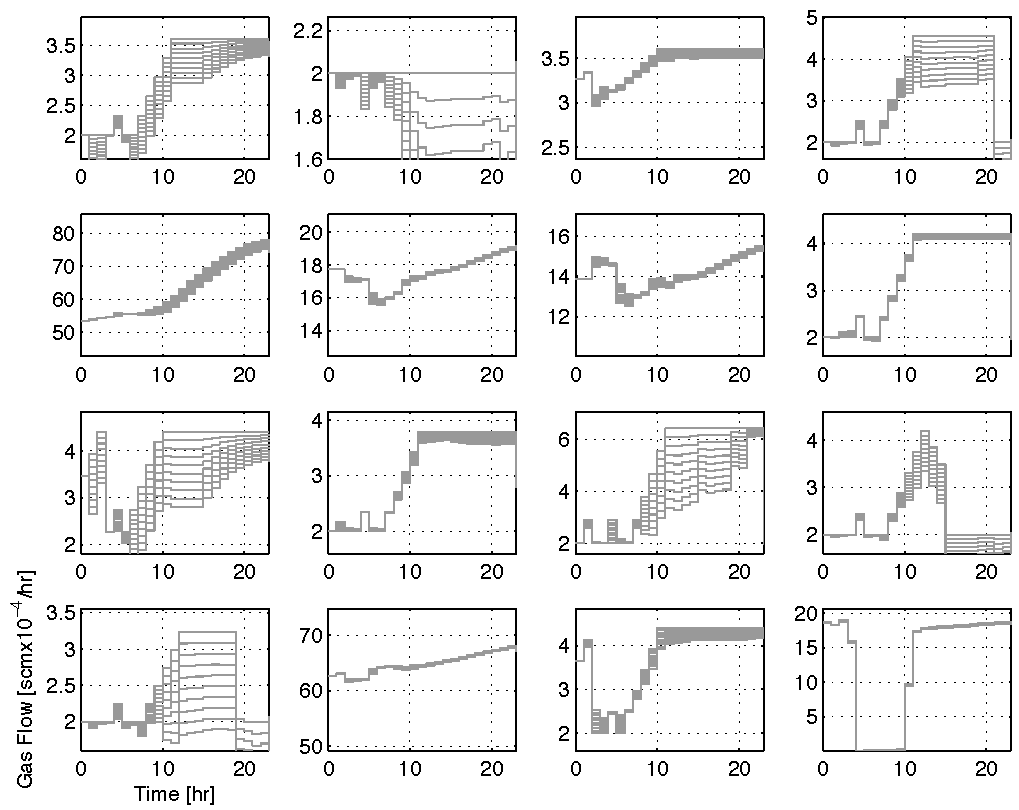
\includegraphics[width=4in]{flow_coupled.pdf}\caption{Spatiotemporal flow profiles for 16 different pipeline segments for coordinated setting.}\label{flow_coupled}
\end{center}
\end{figure}

\subsection{Computational Issues}

We now discuss issues related to the implementation and solution of the optimal control model. 

\subsubsection{Model Implementation}

We discretize the continuous-time grid model \eqref{eq:grid} using an implicit Euler discretization scheme. We discretize the gas model \eqref{eq:gas} in time using an implicit Euler scheme and in space using a forward finite-difference scheme. The discretized power grid problem is a linear program, wheres the discretized gas problem is a nonlinear programming problem (NLP).  The coupled problem is an NLP.  We implement the coupled and decoupled models independently using the algebraic modeling language AMPL. The use of an algebraic modeling language is key because it enables us to obtain exact first and second-order derivative information for the gas model.  Exact derivatives are essential for efficient handling problems with many degrees of freedom as those arising in interconnected models \cite{zavalapavia}. 


\subsubsection{Model Solution}

We solved the coupled and uncoupled models using a 24-hour time horizon with 1-hour time resolution. In our base implementation we discretize each pipeline segment using $N_x=10$ finite-difference points. This gives rise to an optimal control problem with 2,400 differential equations, 2000 algebraic equations, and 1040 controls.  After full discretization, the coordinated problem \eqref{eq:struct} is an NLP with 249,919 variables, 224,292 equality constraints, and 154,093 inequality constraints.  The problem has a total of 25,627 degrees of freedom. 

The computational results are summarized in Table \ref{table:compu}. The solution time for the base problem is approximately 40 minutes.  While the results are acceptable for off-line analysis, such times are too long to consider an actual real-time implementation of the model (which would probably need to be solved every 5 minutes to be compatible with current economic dispatch practices).  The long solution times are partially attributed to the high nonlinearity of the gas network model which induces negative curvature. In the presence of negative curvature, the Hessian of the Lagrangian needs to be regularized (convexified) several times during the search and each regularization attempt requires an additional factorization. In particular, in Table \ref{table:compu} we can see that the total number of iterations is 232 while the total number of factorizations is 311, which indicates that 79 regularization attempts are needed. 

We also attribute the long solution times to the complexity of the linear algebra system. In particular, we noticed that MA57 introduced a significant amount of fill-in, an indication of tight connectivity of the algebraic equations. We attribute this to the complexity induced by the PDAEs coupled with the network equations. To confirm this observation, we performed an additional experiment in which we {\em perturbed the gas network topology by eliminating a single pipeline.} This action splits the Illinois gas network into two independent subnetworks (the power grid topology remains intact). The results for the base and the perturbed topologies are presented in Table \ref{table:compu}. The time per iteration is decreased by 18\% under the perturbed topology.  We also note a significant reduction in the number of iterations and regularizations which indicates that the nonlinearity is ameliorated with a change in topology. In particular, for the base topology we require 311/232=1.34 regularizations per iteration, whereas for the perturbed topology we require 153/136=1.125.  

\begin{table}[htp]
\small
\caption{Computational results for coupled problems for base and perturbed topologies.}
\begin{center}
\begin{tabular}{lcccccc}
                  & Iter. & Solution Time [sec] & Factorizations [-] & Time/Factorization [sec]\\
\hline {\bf Base Topology}  ($N_x=10$)&  232 & 2401.01 & 311 & 7.72\\
{\bf Perturbed Topology} ($N_x=10$)&   136 & 968. 47&  153  & 6.32\\
{\bf Base Topology} ($N_x=3$)&   157 & 573.68&  188   &3.05                      
\end{tabular}
\end{center}
\label{table:compu}
\end{table}%

We next analyze the effects of the discretization resolution on the model results. We compare the results using our base implementation with $N_x=10$ spatial points per pipeline and a low resolution implementation with $N_x=3$ spatial points per pipeline. This low-resolution problem is an optimal control problem with 2,800 DAEs and 1,040 controls. After full discretization, this gives an NLP with 141,559 variables, 115,932 equality constraints, and 157,765 inequality constraints. The problem has a total of 25,627 degrees of freedom (the number of controls is the same as in the base case). The number of degrees of freedom remains unchanged because all of these enter at the network nodes and are thus independent of the discretization resolution \cite{zavalastochgas}. This is an important structural property of gas networks. The results comparing high and low resolutions are presented in Table \ref{table:compu}. The solution time is reduced from 40 minutes to about 10 minutes. Decreasing the resolution decreases both the number of regularizations to 1.19 (compared with 1.34 in the base case) and the time per factorization by a factor 2.5.  

We also compare the economic performance of the low- and high-resolution models for the coordinated and uncoordinated settings. The results are presented in Table \ref{table:reso}. The amount of compression power in the uncoordinated case is underestimated by 21\%, but the impacts on the rest of the metrics are not significant.  This indicates that a low discretization resolutions can adequately capture the overall system behavior and can be used to obtain approximate solutions. Despite these improvements, however, we can see that state-of-the-art tools hit their limits of performance on small regional-scale networks and will not be capable of handling ISO-sized domains.  Based on the estimates obtained for the Illinois system, we anticipate such NLPs to have tens of millions of variables and constraints. Specialized techniques based on decomposition and adaptive discretizations are needed to address models of this magnitude.  
\begin{table}[htp]
\footnotesize
\caption{Economic performance under low- and high-resolution discretizations.}
\begin{center}
\begin{tabular}{lcccccc}
                                         &$ \varphi^{grid}$ [M\$] &$ \varphi^{gas}$ [M\$] & $ \varphi^{gas,comp}$ [\$]  & $d^{gas,target} $[scm $\times10^{-6}$] & $d^{gas}$ [scm$\times 10^{-6}$] & $\mathcal{R}^{gas}$ [M\$]\\
\hline {\bf Uncoord} ($N_x=10$) &         36.54              &        -13.52             &         28,618           &  141.25                & 135.54          & 2.70\\
{\bf Uncoord} ($N_x=3$) &         36.51              &        -13.57             &         23,592           &  141.12                & 135.96          & 2.74\\
\hline {\bf Coord} ($N_x=10$)               &        36.40              &        -14.54             &         33,600           &  145.74               &  145.74          & 3.50 \\
{\bf Coord} ($N_x=3$)                &        36.39              &        -14.55             &         33,356           &  145.83               &  145.83          & 3.48 
\end{tabular}
\end{center}
\label{table:reso}
\end{table}

%%%%%%%%%%%%%%%%%%%%%%%%%%%%%%%%%%%%%%%%%%

\section{Conclusions}

We have presented an optimal control model for integrated gas-electric infrastructures. We used the model to demonstrate that significant improvements in economic performance and flexibility can be gained by coordinated dispatch.  Using a large-scale study we demonstrated that, under a coordinated setting, it is possible to deliver significantly larger amounts of  gas to the power grid and to improve the revenue of gas-fired plants. We observe that, under a coordinated setting, power plants act as controllable demand response resources that can be used by the gas pipeline operator to better control pressure and flows in space and time. This allows the gas operator to bypass delivery bottlenecks. We also used our model to illustrate that power dispatch policies can strongly influence the flow dynamics of the gas infrastructure.  In addition, we found that the state-of-the-art tools can adequately address regional-scale networks but are insufficient to address national-scale networks.  As part of future work, we will develop scalable linear algebra strategies based on decomposition and multi-grid techniques to address such problems.  We will also develop models that capture transient stability of the power grid and that capture other dependencies between infrastructures. For instance, we will model dual-drive compressors that can run on both natural gas and electricity.  

%%%%%%%%%%%%%%%%%%%%%%%%%%%%%%%%%%%%%%%%%%

\section*{Acknowledgments}
This material is based upon work supported by the U.S. Department of Energy, Office of Science, under Contract
No. DE-AC02-06CH11357.

%%%%%%%%%%%%%%%%%%%%%%%%%%%%%%%%%%%%%%%%%%

\bibliography{vzavala}

\end{document}
